One of the major focuses of this work has been a completely new implementation of a program to generate and analyse $SU(3)$ lattice gauge field configurations. As it is common practice in Lattice QCD numerical implementations, the program is split in three parts:
\begin{enumerate}
    \item \textit{Generation of Gauge Fields}: in this case it is done using an implementation of the Metropolis algorithm using the gluonic Wilson action;
    \item \textit{Computation of Lattice Observables}: this includes applying the gradient flow to the gauge fields, as well as computing the energy density and the topological charge at every flow time; in other applications the computation of quark propagators and two- or three-point correlators are performed; 
    \item \textit{Computation of Derived Quantities}: mainly post analysis, computation of secondary observables and uncertainties. Resampling and autocorrelation analysis are crucial to Lattice QCD given the typically small size of the ensembles. 
\end{enumerate}
In this chapter the main features of the first two steps, which are the most interesting, will be presented. The first two points are numerically very challenging and the calculations had to be performed on computing clusters. The third, the post analysis, is a simpler calculation, so regular tabletop computers could be exploited. \\
The programming language of choice was \cpp because of its high efficiency, high abstraction capabilities (the code-base is highly object oriented and extensive use of operator overloading was involved) and for the easiness of the \mpi integration. The analysis of data has been performed using \texttt{python} and in particular relying heavily on its standard data science packages such as \texttt{numpy} and \texttt{pandas}.
  
\section{Generating Pure Gauge Fields}
The task of generating lattice field configurations is extremely demanding in terms of computation requirements. The case of QCD is much more demanding than that of a pure gauge theory, but overall the latter calculation is still challenging. The main, and perhaps overwhelmingly simple, reason for this problem is the dimensionality. Dealing with a discretized space-time lattice, things tend to scale with powers of $2^4$, a trivial example is cutting in half the lattice spacing keeping a fixed total volume: this requires $16$ more points in the global lattice. \\
To get a better feeling of the algorithm we first have to look at what the basic object of the program is: the lattice. On a computer the number of double precision floating point numbers to be stored for a field configuration is given by
\begin{equation}
    \underbrace{N^3}_\text{spatial dimension} \times
    \underbrace{N_t}_\text{time dimension} \times
    \underbrace{4}_\text{links per site} \times 
    \underbrace{9}_\text{SU(3) matrix size} \times
    \underbrace{2}_\text{real and imaginary part}
\end{equation}
For example, if we choose $N=48,~N_t=96$ (which is the largest system considered in this work) the resulting configuration is $6115295232~bytes$ large, that is $5.7~GBytes$.  The incredibly large size of the data to be handled limits greatly the possibility of simulating larger systems. \\
The basic element at each lattice site is a set of $4$ different $SU(3)$ matrices, one for each dimension, these are the links variables described in \cref{sec:lattice_discretize}. Since the links with negative orientation are related to the ones with positive orientation by the adjoint operation, only the postively oriented ones are stored in memory.  

\subsection{The Metropolis Algorithm}
The main algorithm that has been used to generate an ensemble of gauge field configurations is the Metropolis Algorithm. It is a widely popular Markov Chain Monte Carlo Method to generate a sequence of random samples from a probability distribution \cite{metropolis_equation_1953}\cite{mhj}. \\
In general, a Markov Chain is a a sequence randomly chosen variables $X_1, X_2, \dots, X_t$, in our case a lattice field configuration, with the Markov Property, that is: the probability of the step $t+1$ depends only on the variable $X_t$:
\beq
    P(X_{t+1} = x| X_1 = x_1, X_1 = x_2, \dots, X_t = x_t) = P(X_{t+1} = x|  X_t = x_t) 
\eeq 
In the case where the probabilities of moving from a state $X_i = i$ to a state $X_j = j$ is not known, the transition probability from the two states, $W(i\rightarrow j)$ can be split into two contributions: the probability $T(i \rightarrow j)$ for making the transition to state $j$ being in state $i$ and the the probability of accepting this transition $A(i \rightarrow j)$.
\beq
    W(i \rightarrow j) = A(i \rightarrow j)T(i \rightarrow j)
\eeq  
If a Probability Distribution Function (PDF) is known for the process, we can label the probability of a given state at a fixed time $w_i(t)$. The transition probability to a state $j$ at time $t+1$ is the sum of the transition probabilities of moving to state $j$ from state $i$ plus the probability of being in state $i$ at time $t$ and rejecting to move to any other state:
\begin{align}
    w_{j} (t+1) &= \sum_i \left[ w_i(t)T(i\rightarrow j)A(i\rightarrow j) + w_j(t)T(j\rightarrow i)\left(1-A(j\rightarrow i)\right)  \right]\\\nonumber
    &=  w_j(t) + \sum_i \left[ w_i(t)T(i\rightarrow j)A(i\rightarrow j) -  w_j(t)T(j\rightarrow i)A(j\rightarrow i)  \right]
\end{align}
for large $t$, when the equilibrium is reached, we require that $w_{j} (t+1) = w_{j} (t) = w_j$, and thus we have:
\beq
    \sum_i w_iT(i\rightarrow j)A(i\rightarrow j) =  \sum_i w_jT(j\rightarrow i)A(j\rightarrow i) 
\eeq 
now, considering that the transition probability from a state $j$ to all other states must be normalized $\sum_i W(j\rightarrow i)  = \sum_i T(j\rightarrow i)A(j\rightarrow i) = 1$ we get:
\beq
    \sum_i w_iT(i\rightarrow j)A(i\rightarrow j) =  w_j
\eeq 
At this point, the further constrain of Detailed Balance is introduced, that is:
\beq
    w_iW(i\rightarrow j) =  w_j W(j\rightarrow i)
\eeq 
at equilibrium we then have:
\beq
    \frac{w_i}{w_j} = \frac{W(i\rightarrow j)}{W(j\rightarrow i)} = \frac{T(i\rightarrow j)A(i\rightarrow j)}{T(j\rightarrow i)A(j\rightarrow i)}
\eeq
Making the approximation that the transition probability between states is the same, $T(i\rightarrow j) = T(j\rightarrow i)$, the brute-force approach, we are left with the acceptance ratio of a move to an new state to be the ratio of the PDFs.  

In the case of pure gauge fields, the probability distribution is:
\beq
\label{eq:PDF}
    P(U) = \frac{e^{S_G[U]}}{Z} = \frac{e^{S_G[U]}}{\int \D ~U e^{S_G[U]} }
\eeq
which is the exponential of gluon Wilson Action over the path integral of the same quantity over all space (the partition function). Luckily, we only need ratios of PDFs so the partition functions is not to be computed. We can rewrite any expectation value of an operator on the lattice as:
\beq
    \langle O \rangle = \frac{\int \D U ~O[U] e^{S_G[U]}}{\int \D ~U e^{S_G[U]} } = \int  \D U ~ P(U) O[U]
\eeq
which numerically becomes:
\beq
\langle O \rangle \approx \frac{1}{N} \sum_{i=1}^N O(U_i)
\eeq
where, as described in section \cref{sec:pathintegral} $U_i$ are random configurations of a set chosen with the PDF in \cref{eq:PDF}. \\
Noting that, since we only care about ratios in the PDF, which turn out to be exponentials of the action difference between to configurations,  a tentative algorithm can be written as: 
\begin{algorithm} [hbt!]
    \caption{Metropolis Algorithm}\label{metropolis:algo}
    \begin{algorithmic}
    \State $\textit{configuration} \gets \text{initial configuration}$
    \For {$i < \textit{MonteCarloCycles}$}
        \For {$j < N_{corr}$}
            \For {$U$ in \textit{Lattice}}
                \State $\textit{newConfiguration}  \gets \text{randomMove}(U) + \textit{configuration}$  
                \State $\Delta S \gets \text{action} (\textit{newConfiguration}) - \text{action} (\textit{configuration})$
                \If {$\Delta S > random(0,1)$} 
                    \State $\textit{configuration} \gets \textit{newConfiguration}$
                \EndIf
            \EndFor 
        \EndFor 
        \State saveConfiguration$(configuration)$
    \EndFor
    \end{algorithmic}  
\end{algorithm} 

The actual implementation of this algorithm on discretized space-time is however not as trivial as it seems. Firstly, a definition of what is a ``random move'' in configuration space is needed, secondly an efficient way of computing the action difference is to be found.

The ensemble, on which observables can be computed, is created by saving to disk, in the form of a simple binary file containing all the data,  one configuration every $N_C$ Monte Carlo updates. We need this in order to apply the gradient flow afterwards to the configurations and compute the observables we want. The choice of $N_C$ turned out to be crucial for the autocorrelation of some observables, in particular the topological charge, see \cref{sec:testautocorr}.

\subsection{Sampling the Configuration Space}
To use Metropolis' algorithm we need to define what a random move is. Using the Wilson Action \cref{intro:lat_action}, which is defined on plaquettes, an random move in the configuration space, on a single link variable, can be seen as a small unitary transformation in the $SU(3)$ group. By small it is intended that the unitary matrix has a strong real diagonal component, making it close to an identity matrix. In order to generate such transformation we use three random $SU(2)$ matrices that are as well ``close to unity''. A recipe for generating these matrices is found in \cite{gattringer_quantum_2010}. We consider three $2\times 2$ unitary matrixes $R_2,S_2$ and $T_2$:
\beq
    R_2 = \begin{pmatrix}
        r_{11} & r_{12} \\ r_{21} & r_{22} 
    \end{pmatrix}
    ~~~~~~~
    S_2 = \begin{pmatrix}
        s_{11} & s_{12} \\ s_{21} & s_{22} 
    \end{pmatrix}
    ~~~~~~~
    T_2 = \begin{pmatrix}
        t_{11} & t_{12} \\ t_{21} & t_{22} 
    \end{pmatrix}
\eeq
The elements of the matrix are to be random but with a controlled spread around the identity matrix. One starts by selecting four random numbers $r_0$, $\vec{r}$ (the latter is a three component vector) between $(-\frac{1}{2},\frac{1}{2})$. 
Then a ``spread parameter'' $\epsilon$ is introduced, which controls how much the off-diagonal terms will weight. The random variables are scaled according to:
\beq
    x_0 = sign(r_0)\sqrt{1-\epsilon^2}~~~~~~\vec{x} = \epsilon \frac{\vec{r}}{|\vec{r}|}
\eeq
and these four coefficients, together with the generators of the $SU(2)$ group (the Pauli matrices)  are used to build the element of the group:
\beq
U = x_0\mathds{1} + i\vec{x}\cdot\vec{\sigma} = \begin{pmatrix}
    u_{11} & u_{12} \\ u_{21} & u_{22} 
\end{pmatrix}
\eeq
One then embeds these $SU(2)$ matrices in three $SU(3)$ matrices by mapping them as:
\beq
    R = \begin{pmatrix}
        r_{11} & r_{12} & 0\\ r_{21} & r_{22} & 0 \\ 0 & 0 & 1 
    \end{pmatrix}
    ~~~~~~~
    S = \begin{pmatrix}
        s_{11} & 0 & s_{12} \\ 0 & 1 & 0 \\ s_{21} & 0 & s_{22} 
    \end{pmatrix}
    ~~~~~~~
    T = \begin{pmatrix}
        1 & 0 & 0 \\ 0 & t_{11} & t_{12} \\ 0 & t_{21} & t_{22} 
    \end{pmatrix}
\eeq
These three matrices are clearly members of the $SU(3)$ group and so is their product $X = RST$, which is used as the ``random move'' in the Metropolis algorithm. We thus have defined a recipe for numerically generating random transformations, the key element for our algorithm.

\subsection{Efficient Action Difference Calculation}
An additional element that is needed is the action difference $\Delta S$. When a random transformation $U_\mu(x) \rightarrow U'_\mu(x) = XU_\mu(x)$ is applied on a single link of the lattice, the total change in the action only depends on those plaquettes that contain the considered link variable. In four dimensions there are 12 such elements:
\beq
    \Delta S = S[U'_\mu(x)] - S[U_\mu(x)]  = -\frac{\beta}{N} \text{Re}~ Tr \left( [U'_\mu(x) - U_\mu(x)] A[U_\mu(x)]\right)
\eeq
where $A[U_\mu(x)]$ is the sum of the "staples" of the link $U_\mu(x)$. They are the constant three sides of the plaquettes that contain $U_\mu(x)$:
\begin{align}
    \label{eq:staples}
    A[U_\mu(x)] = \sum_{\nu\neq\mu} &\bigg[ U_{\nu}(x+\mu)U_{-\mu}(x+\mu+\nu)U_{-\nu}(x+\nu) \\\nonumber
    +  &U_{-\nu}(x+\mu)U_{-\mu}(x+\mu-\nu)U_{\nu}(x-\nu)  \bigg]
\end{align}

\begin{figure}[!htb]
    \centering

    \begin{tikzpicture}[scale=0.7]

        \pgfmathsetmacro\len{1.2};
        \pgfmathsetmacro\startx {-6};
        \pgfmathsetmacro\startxx {-5};
        \pgfmathsetmacro\startxxx {-3};
        \pgfmathsetmacro\startxxxx {0};

        \pgfmathsetmacro\starttxxxx {4.5};
        \pgfmathsetmacro\starttx {4};
        \pgfmathsetmacro\starttxx {4.8};
        \pgfmathsetmacro\starttxxx {6.8};
        \pgfmathsetmacro\starty {0};
        \pgfmathsetmacro\startty {0};

        \node [left] (a) at  (\startx, \starty) {$S[U_\mu] = \sum_{\nu\neq\mu}$}; 
         
        \draw (-5,-2) to [round left paren ] (-5,2);

        % ++
        \draw[->-=.7, >=latex] (\startxx,\starty) to (\startxx+\len,\starty);
        \draw[->-=.7, >=latex] (\startxx+\len,\starty) to  (\startxx+\len,\starty+\len);
        \draw[->-=.7, >=latex] (\startxx+\len,\starty+\len) to (\startxx,\starty+\len);
        \draw[->-=.7, >=latex] (\startxx,\starty+\len) to (\startxx, \starty);
 
        \node (b) at (-3.4, \starty) {$+$}; 
        %+-
        \draw[->-=.7, >=latex] (\startxxx,-\starty) to (\startxxx+\len,-\starty);
        \draw[->-=.7, >=latex] (\startxxx+\len,-\starty) to  (\startxxx+\len,-\starty-\len);
        \draw[->-=.7, >=latex] (\startxxx+\len,-\starty-\len) to (\startxxx,-\starty-\len);
        \draw[->-=.7, >=latex] (\startxxx,-\starty-\len) to (\startxxx, -\starty);
        \draw (-1.7,-2) to [round right paren ] (-1.7,2); 

       \node (c) at  (-0.7, \starty) {$=$}; 

        \draw[->-=.7, >=latex] (\startxxxx,\starty) to (\startxxxx+\len,\starty); 

       \node [right](f) at  (1.4, \starty) {$\times \sum_{\nu\neq\mu} $}; 
         
        \draw (\starttxxxx,-2) to [round left paren ] (\starttxxxx,2);

        % ++
        \draw[->-=.7, >=latex] (\starttxx+\len,\startty) to  (\starttxx+\len,\startty+\len);
        \draw[->-=.7, >=latex] (\starttxx+\len,\startty+\len) to (\starttxx,\startty+\len);
        \draw[->-=.7, >=latex] (\starttxx,\startty+\len) to (\starttxx, \startty);
 
        \node (d) at  (6.4, \startty) {$+$}; 
        %+-
        \draw[->-=.7, >=latex] (\starttxxx,-\startty-\len) to (\starttxxx,-\startty);
        \draw[->-=.7, >=latex] (\starttxxx+\len,-\startty) to  (\starttxxx+\len,-\startty-\len);
        \draw[->-=.7, >=latex] (\starttxxx+\len,-\startty-\len) to (\starttxxx,-\startty-\len);
        \draw (8.2,-2) to [round right paren ] (8.2,2); 

    \end{tikzpicture}

    \capt{Schematic representation of the symmetric definition of action $S[U_\mu]$ expressed as a function of the staples .}
    \label{fig:staples}
\end{figure}


\subsection{Updates Strategies}
There is now some arbitrariness in what is defined as a Monte Carlo update, or cycle. In this work we call an update the procedure outlined in \cref{metropolis:update}. 
\begin{algorithm}[bht!]
    \caption{Metropolis Update}\label{metropolis:update}
    \begin{algorithmic}[1]
    \For {$x,\mu$}
        \State $A \gets computeStaples(x,\mu)$     
        \For {$i < N_{H}$}
            \State $U_{new}(x,\mu)  \gets X\cdot U(x,\mu)$  
            \State $\Delta S \gets (U_{new}(x,\mu)  - U(x,\mu) )\cdot A$
            \If {$realTrace(\Delta S) > random(0,1)$} 
                \State $U(x,\mu)  \gets U_{new}(x,\mu)$
            \EndIf
        \EndFor
    \EndFor
\end{algorithmic}
\end{algorithm}
These updates are the ones we consider when we refer to Monte Carlo cycles in the context of thermalization and autocorrelation time, for example. Note that each update includes a loop over all links on the lattice and that every link is "hit" $N_H$ times before moving to the next one. This is done for computational efficiency, because computing the staples is the most expensive part of the algorithm, once $A$ is computed for a link, the result is used to attempt multiple updates on the link. It can also be shown that if $N_H$ is sufficiently large the algorithm becomes equivalent to the heatbath algorithm. 

The order in which the links in the lattice are visited is also arbitrary. The simplest way, that is iterating on the links as they are stored in memory, was adopted. This however might have impacted the autocorrelation of the system, not allowing significant modification to the system as an update depends on the neighbors. An alternative choice is a checkerboard pattern, which has potential benefits to the autocorrelation time of the observables as well as on the performance, as it allows for better communication patterns in the case of parallelized code. 

\subsection{Parallelization Scheme}
\label{sec:para_gen}
Given the size of the lattice (from $V \approx 10^5$ to $V\approx 10^7$, the total number of lattice sites), it is almost necessary to split the computation of the updates on more than one processors. The most direct way is to divide the lattice into sub-blocks and have each process handle its portion of the field alone. \\
In an operative way, given a lattice of size $(n_x, n_y, n_z, n_t)$ each space-time dimension is split into even portions, of size $(s_x, s_y, s_z, s_t)$ and mapped on $N_{procs}$ processors, having that:
\beq
N_{procs} = \frac{s_x}{n_x} \times \frac{s_y}{n_y} \times \frac{s_z}{n_z}  \times \frac{s_t}{n_t}
\eeq 
A unique mapping can be performed from the ``local'' coordinates of the sub-block and the global coordinates through the aid of the unique identifier of the processor that is given by the parallelization library. In particular, the Message Passing Interface (MPI) has a built-in function to map processors into a grid of arbitrary dimensions and size, called \texttt{MPI\_CartCoord\_Create}. The utility also allows for the ease identification of the rank (the jargon term for the unique identifier of a processor) of the nearest neighbors. Using this tools one can manage the distribution of the total lattice into $N_{procs}$ sub-lattices. \\
However, because of the dependence of the action difference of a link on its neighboring site, when updating a link on the edge of of a sub-block information about another block is needed. Here is where MPI comes in use, substituting the usual periodic boundary conditions that are used in the calculations with periodic communication patterns between the processors. For this particular problem we decided to use a point to point communication scheme, the use of periodic boundary conditions allowed also for non-blocking communications, in particular the collective geometry based scheme shown in \cref{fig:subblocks} has been implemented. 

\newif\ifcuboidshade
\newif\ifcuboidemphedge

\tikzset{
  cuboid/.is family,
  cuboid,
  shiftx/.initial=0,
  shifty/.initial=0,
  dimx/.initial=3,
  dimy/.initial=3,
  dimz/.initial=3,
  scale/.initial=1,
  densityx/.initial=1,
  densityy/.initial=1,
  densityz/.initial=1,
  rotation/.initial=0,
  anglex/.initial=0,
  angley/.initial=90,
  anglez/.initial=225,
  scalex/.initial=1,
  scaley/.initial=1,
  scalez/.initial=0.5,
  front/.style={draw=black,fill=white},
  top/.style={draw=black,fill=white},
  right/.style={draw=black,fill=white},
  shade/.is if=cuboidshade,
  shadecolordark/.initial=black,
  shadecolorlight/.initial=white,
  shadeopacity/.initial=0.15,
  shadesamples/.initial=16,
  emphedge/.is if=cuboidemphedge,
  emphstyle/.style={thick},
}

\newcommand{\tikzcuboidkey}[1]{\pgfkeysvalueof{/tikz/cuboid/#1}}

% Commands
\newcommand{\tikzcuboid}[1]{
    \tikzset{cuboid,#1} % Process Keys passed to command
  \pgfmathsetlengthmacro{\vectorxx}{\tikzcuboidkey{scalex}*cos(\tikzcuboidkey{anglex})*28.452756}
  \pgfmathsetlengthmacro{\vectorxy}{\tikzcuboidkey{scalex}*sin(\tikzcuboidkey{anglex})*28.452756}
  \pgfmathsetlengthmacro{\vectoryx}{\tikzcuboidkey{scaley}*cos(\tikzcuboidkey{angley})*28.452756}
  \pgfmathsetlengthmacro{\vectoryy}{\tikzcuboidkey{scaley}*sin(\tikzcuboidkey{angley})*28.452756}
  \pgfmathsetlengthmacro{\vectorzx}{\tikzcuboidkey{scalez}*cos(\tikzcuboidkey{anglez})*28.452756}
  \pgfmathsetlengthmacro{\vectorzy}{\tikzcuboidkey{scalez}*sin(\tikzcuboidkey{anglez})*28.452756}
  \begin{scope}[xshift=\tikzcuboidkey{shiftx}, yshift=\tikzcuboidkey{shifty}, scale=\tikzcuboidkey{scale}, rotate=\tikzcuboidkey{rotation}, x={(\vectorxx,\vectorxy)}, y={(\vectoryx,\vectoryy)}, z={(\vectorzx,\vectorzy)}]
    \pgfmathsetmacro{\steppingx}{1/\tikzcuboidkey{densityx}}
  \pgfmathsetmacro{\steppingy}{1/\tikzcuboidkey{densityy}}
  \pgfmathsetmacro{\steppingz}{1/\tikzcuboidkey{densityz}}
  \newcommand{\dimx}{\tikzcuboidkey{dimx}}
  \newcommand{\dimy}{\tikzcuboidkey{dimy}}
  \newcommand{\dimz}{\tikzcuboidkey{dimz}}
  \pgfmathsetmacro{\secondx}{2*\steppingx}
  \pgfmathsetmacro{\secondy}{2*\steppingy}
  \pgfmathsetmacro{\secondz}{2*\steppingz}
  \ifthenelse{\equal{\dimx}{1}}
    {\foreach \x in {\steppingx,...,\dimx}}
    {\foreach \x in {\steppingx,\secondx,...,\dimx}}
  {     \ifthenelse{\equal{\dimy}{1}}
    {\foreach \y in {\steppingy,...,\dimy}}
    {\foreach \y in {\steppingy,\secondy,...,\dimy}}
    {   \pgfmathsetmacro{\lowx}{(\x-\steppingx)}
      \pgfmathsetmacro{\lowy}{(\y-\steppingy)}
      \filldraw[cuboid/front] (\lowx,\lowy,\dimz) -- (\lowx,\y,\dimz) -- (\x,\y,\dimz) -- (\x,\lowy,\dimz) -- cycle;
    }
    }
    \ifthenelse{\equal{\dimx}{1}}
    {\foreach \x in {\steppingx,...,\dimx}}
    {\foreach \x in {\steppingx,\secondx,...,\dimx}}
  { \ifthenelse{\equal{\dimz}{1}}
    {\foreach \z in {\steppingz,...,\dimz}}
    {\foreach \z in {\steppingz,\secondz,...,\dimz}}
    {   \pgfmathsetmacro{\lowx}{(\x-\steppingx)}
      \pgfmathsetmacro{\lowz}{(\z-\steppingz)}
      \filldraw[cuboid/top] (\lowx,\dimy,\lowz) -- (\lowx,\dimy,\z) -- (\x,\dimy,\z) -- (\x,\dimy,\lowz) -- cycle;
        }
    }
    \ifthenelse{\equal{\dimy}{1}}
    {\foreach \y in {\steppingy,...,\dimy}}
    {\foreach \y in {\steppingy,\secondy,...,\dimy}}
  { \ifthenelse{\equal{\dimz}{1}}
    {\foreach \z in {\steppingz,...,\dimz}}
    {\foreach \z in {\steppingz,\secondz,...,\dimz}}
    {   \pgfmathsetmacro{\lowy}{(\y-\steppingy)}
      \pgfmathsetmacro{\lowz}{(\z-\steppingz)}
      \filldraw[cuboid/right] (\dimx,\lowy,\lowz) -- (\dimx,\lowy,\z) -- (\dimx,\y,\z) -- (\dimx,\y,\lowz) -- cycle;
    }
  }
  \ifcuboidemphedge
    \draw[cuboid/emphstyle] (0,\dimy,0) -- (\dimx,\dimy,0) -- (\dimx,\dimy,\dimz) -- (0,\dimy,\dimz) -- cycle;%
    \draw[cuboid/emphstyle] (0,\dimy,\dimz) -- (0,0,\dimz) -- (\dimx,0,\dimz) -- (\dimx,\dimy,\dimz);%
    \draw[cuboid/emphstyle] (\dimx,\dimy,0) -- (\dimx,0,0) -- (\dimx,0,\dimz);%
    \fi

    \ifcuboidshade
    \pgfmathsetmacro{\cstepx}{\dimx/\tikzcuboidkey{shadesamples}}
    \pgfmathsetmacro{\cstepy}{\dimy/\tikzcuboidkey{shadesamples}}
    \pgfmathsetmacro{\cstepz}{\dimz/\tikzcuboidkey{shadesamples}}
    \foreach \s in {1,...,\tikzcuboidkey{shadesamples}}
    {   \pgfmathsetmacro{\lows}{\s-1}
        \pgfmathsetmacro{\cpercent}{(\lows)/(\tikzcuboidkey{shadesamples}-1)*100}
        \fill[opacity=\tikzcuboidkey{shadeopacity},color=\tikzcuboidkey{shadecolorlight}!\cpercent!\tikzcuboidkey{shadecolordark}] (0,\s*\cstepy,\dimz) -- (\s*\cstepx,\s*\cstepy,\dimz) -- (\s*\cstepx,0,\dimz) -- (\lows*\cstepx,0,\dimz) -- (\lows*\cstepx,\lows*\cstepy,\dimz) -- (0,\lows*\cstepy,\dimz) -- cycle;
        \fill[opacity=\tikzcuboidkey{shadeopacity},color=\tikzcuboidkey{shadecolorlight}!\cpercent!\tikzcuboidkey{shadecolordark}] (0,\dimy,\s*\cstepz) -- (\s*\cstepx,\dimy,\s*\cstepz) -- (\s*\cstepx,\dimy,0) -- (\lows*\cstepx,\dimy,0) -- (\lows*\cstepx,\dimy,\lows*\cstepz) -- (0,\dimy,\lows*\cstepz) -- cycle;
        \fill[opacity=\tikzcuboidkey{shadeopacity},color=\tikzcuboidkey{shadecolorlight}!\cpercent!\tikzcuboidkey{shadecolordark}] (\dimx,0,\s*\cstepz) -- (\dimx,\s*\cstepy,\s*\cstepz) -- (\dimx,\s*\cstepy,0) -- (\dimx,\lows*\cstepy,0) -- (\dimx,\lows*\cstepy,\lows*\cstepz) -- (\dimx,0,\lows*\cstepz) -- cycle;
    }
    \fi 

  \end{scope}
}

\makeatother


\begin{figure}[!hbt]
\centering
\begin{tikzpicture}[scale=0.7]

\tikzcuboid{dimx=1,dimy=1,dimz=1,shiftx=-400, scale=4};
\tikzcuboid{dimx=4,dimy=4,dimz=4,shiftx=4,scale=1};
 
\node (A) at (-7, 1) {};
\node (B) at (-4, 1) {};
\draw[-latex,thick] (A) to (B); 
\draw [-latex] (-9.5,2.5) arc [start angle=-45, end angle=225, x radius=4.5cm, y radius=1.3cm];

\draw [-latex] (2.95, 2.1) arc [start angle=-45, end angle=225, x radius=3cm, y radius=1.3cm];


\node (C) at (-12.5, 5.5) {Periodic Boundary Conditions};
\node (D) at (1.6, 5.5) {Periodic Communication Pattern};

\draw [black,decorate,decoration={brace,amplitude=5pt,mirror}](-1.35,-1.55) -- (-0.15,-1.55) node[black,midway,yshift=-0.5cm] {\footnotesize $s_x$ Lattice Sites};

\draw [black,decorate,decoration={brace,amplitude=5pt,mirror}](-15.5,-1.55) -- (-11.5,-1.55) node[black,midway,yshift=-0.5cm] {\footnotesize $n_x$ Lattice Sites};

\draw[-latex] (-0.55, 2.1) to (0.05, 2.1);
\draw[-latex] (-0.55 + 1, 2.1) to (0.05 + 1., 2.1);
\draw[-latex] (-0.55 + 2, 2.1) to (0.05 + 2, 2.1);

\draw[-latex] (-0.55, 1.1) to (0.05, 1.1);
\draw[-latex] (-0.55 + 1, 1.1) to (0.05 + 1., 1.1);
\draw[-latex] (-0.55 + 2, 1.1) to (0.05 + 2, 1.1);

\draw[-latex] (-0.55, 0.1) to (0.05, 0.1);
\draw[-latex] (-0.55 + 1, 0.1) to (0.05 + 1., 0.1);
\draw[-latex] (-0.55 + 2, 0.1) to (0.05 + 2, 0.1);

\draw[-latex] (-0.55, -0.9) to (0.05, -0.9);
\draw[-latex] (-0.55 + 1, -0.9) to (0.05 + 1., -0.9);
\draw[-latex] (-0.55 + 2, -0.9) to (0.05 + 2, -0.9);

\end{tikzpicture}
\label{fig:subblocks}
\capt{Schematic representation, in just 3 dimesnions, of the splitting of the lattice into sub-lattices.}
\end{figure}


When computing the staples, two links need to be fetched from the neighboring sites \NOTE{FIGURE?}, since all processors are synchronized, when one processor is in need of these link variables one of its neighbors is requesting the corresponding links from it. The \texttt{SendRecv} function of MPI is exactly what is needed: it automatically handles, in the most efficient way, multiple data transfer between processors in situations when a single core needs to send and receive from different ranks. \\ 
Note that the communication is relevant only for the computation of the staples, this is another argument in favor of performing multiple hits on a link at every update. It is clear to see that the algorithm can be affected by large communication overhead problems. If the sub-blocks are too small, then most of the time would be spent on sending and receiving links from the neighbors. This causes the execution time to depend not linearly on the number of processors, instead the relation flattens at some value given by the communication overhead.

\subsection{Summary of the Parameters for Generating Configurations}
In total the algorithm has four parameters as inputs. Of these, only one defines the physics of the system, the others have to be set and optimized in order to improve the acceptance ratio of the metropolis algorithm and the autocorrelation of the observables computed on the generated configurations.

\begin{table}[!htb]
\begin{center}
\begin{tabular}{cl}
    Parameter & Description\\\hline
    $\beta$ & Coupling parameter of the Wilson Action\\
    $\epsilon$ & ``Spread'' of the random $SU(3)$ elements for the updates\\
    $N_C$ & Number of updates between one saved configuration (observable measurement)\\
    $N_H$ & Number of of "hits" per link at every update, with constant staple 
\end{tabular}
\label{MC:params}
\capt{Parameters for the Monte Carlo generation of Yang-Mills gauge field configurations via the Metropolis Algorithm}
\end{center}
\end{table}

\section{Gradient Flow of Gauge Configurations}
To study the flow time dependence of the observables a numeric implementation of \cref{lattice:flow} is needed. The main challenge that this problem poses is how to numerically integrate the flow equation on the lattice, because it is important to preserve the $SU(3)$ Lie Group structure of the field through the numerical procedure. The problem is solved by using the so called Structure-Preserving Runge-Kutta Methods, in particular the Runge-Kutta Munthe-Kaas method that is designed to integrate first order ODE on a manifold \cite{munthe-kaas_runge-kutta_1998,munthe-kaas_lie-butcher_1995,celledoni_introduction_2014}. In \cref{algo:flow} the general scheme of the program to flow the gauge field configurations is outlined.
\begin{algorithm}[bht!]
    \caption{Gradient Flow}\label{algo:flow}
    \begin{algorithmic}[1]
    \For {\textit{conf} in $ensemble$}
        \State \textit{conf} \gets readInputFile()     
        \For {$t = 0,~ t_f < t_f^{MAX}$}
            \State $conf$ \gets flowStep(\textit{conf})
            computeObservables(\textit{conf}) 
            \State $t_f$ \gets $t_f + \epsilon$
        \EndFor
    \EndFor
\end{algorithmic}
\end{algorithm}

The main idea is to loop over all the configurations in an ensemble and for each of them numerically integrate in steps of $\epsilon$ (a dimensionless small step parameter) from $t_f=0$ to $t_f = t_f^{MAX}$. By using an explicit RK method, only one lattice is stored in memory at a time, and is updated at every iteration. At each step, the expectation values of all the desired observables are computed and their value stored to file for further analysis.

\subsection{Numerical Integration of the Flow Equation}
The problem of the gradient flow can be defined in more general terms as:
\beq
    \dot{V}_t =  Z(V_t)V_t
\eeq
here $V_t$ is an element of a Lie group $\mathcal{G}$ and $Z(V_t)$ is a function with values in the associated algebra $\mathfrak{g}$, in our case we have $Z(V_t) = -g_0^2\partial_\mu V(t_f)$. The general ansatz for the RK-MK method is to write the integration step, with $\epsilon$ the integration step,  as:
\beq
    V_{t+\epsilon} =  \exp[\epsilon\Omega(V_t)] V_t
\eeq
where $\Omega(V_t)$ is a linear combination of $Z(V_t + \epsilon c_i)$, with $c_i$ the RK coefficients, and of their commutators. 
Following the suggestion of \cite{luscher_properties_2010} and considering the analysis of \cite{ce_non-gaussianities_2015} that suggests that, for a fixed step size, an integrator of third order is sufficient, the integration scheme that has been used is the one found in L{\"u}scher's article:
\begin{align}
    \label{eq:integrator}
    W_0 &= V_t\\\nonumber
    W_1 &= \exp\left[ \frac{1}{4}Z_0 \right] W_0 \\\nonumber
    W_2 &= \exp\left[ \frac{8}{9}Z_1 - \frac{17}{36}Z_0 \right] W_1\\\nonumber
    V_{t+\epsilon} &= \exp\left[ \frac{3}{4}Z_2 - \frac{8}{9}Z_1 + \frac{17}{36}Z_0\right] W_2
\end{align}
where the shorthand notation $Z_i = i\epsilon Z(W_i)$ has been introduced. The choice of the coefficients for the Butcher's tableu of the RK method is made in order to satisfy the requirements for a third order RK integrator and to cancel the commutator terms in $\Omega(V_t)$ when expanding it with the Baker-Campbell-Husdorff formula. \\
What is then left to define are the derivative of the action at a given lattice site and the numerical exponentiation of a member of the $\mathfrak{su}(3)$ algebra, which returns an $SU(3)$ element.

\subsection{The Action Derivative}
The differential operator acting on an algebra-valued function $f(U)$ in a Lie group is defined, in terms of the generators $t^a$:
\beq
    \partial_{\mu,x}^a f(U) = \frac{d}{ds} f(e^{sX}U) \bigg\rvert_{s=0},~~~~~\text{with} ~~~X(\mu,x) = t^a \delta_{x,y}\delta_{\mu,\nu} 
\eeq
In practice this operator leaves unchanged all the links except the one that is being derived. When considering the action in \cref{wilsonaction} and recalling the definition of staples \cref{eq:staples} we have:
\beq
\partial_{\mu,x}^a S_G(U_\mu(x)) = -\frac{2}{g_0^2} \sum_{x \in \Lambda} \sum_{\mu \neq \nu} \text{Re}\Tr (1-P_{\mu\nu}) = -\frac{2}{g_0^2}  \text{Re}\Tr (t^a U_\mu(x) A[U_\mu(x)])
\eeq
Defining $\Omega_\mu(x) = U_\mu(x) A[U_\mu(x)]$ and summing over all generators one has:
\beq
g_0^2\partial_{\mu,x} S_G(U_\mu(x)) = 2 t^a  \text{Re}\Tr (t^a \Omega_\mu(x)) = t^a \Tr (t^a (\Omega_\mu(x) - \Omega^\dagger_\mu (x)) 
\eeq
Invoking now the fact that any $3\times3$ matrix can be expanded as $M = \frac{1}{3} \Tr M - 2 t^a\Tr(t^aM)$, inverting this relation we get:
\beq
g_0^2\partial_{\mu,x} S_G(U_\mu(x)) = \frac{1}{2} \left(\Omega_\mu(x) - \Omega^\dagger_\mu (x) \right) -  \frac{1}{6} \Tr \left(\Omega_\mu(x) - \Omega^\dagger_\mu (x) \right)
\eeq
that is our final expression for the action derivative. It should be noticed that computing this term is not anymore complex than computing the action difference for the gauge field configuration generation case, as in both cases the most complicated object to calculate on the lattice is the sum of the staples. We can notice as well that the derivative is always a traceless hermitean matrix, thus an element of $\mathfrak{su}(3)$ as expected.

\subsection{Exponential of a $\mathfrak{su}(3)$ Element}
The last thing to define from \cref{eq:integrator} is how to exponentiate the action derivative. Following \cite{morningstar_analytic_2004} we provide a numerical recipe for taking the exponential function of a traceless hermitean $3\times3$ matrix. The key idea is to use the Cayley-Hamilton theorem, that states that every matrix is a zero of its characteristic polynomial:
\beq
    Q^3 - c_1 Q - c_0\mathds{1} = 0,~~~~~\text{with}~~c_0 = \det Q = \frac{1}{3}(Q^3),~~~c_1 =\frac{1}{2}(Q^2)
\eeq
The exponential of $iQ$ can then be written as:
\beq    
e^{iQ} = f_0\mathds{1} + f_1Q+f_2Q^2
\eeq
where the functions of the eigenvalues of $Q$, which in turn can be parameterized, because of the hermitianeity of $Q$ in terms of $c_0$ and $c_1$. Labeling the eigenvalues of $Q$ as $q_1, q_2, q_3$ and using the fact that the matrix is traceless they can be parametrized as:
\beq
    q_1 = 2u~~~~~~~q_2 = -u+w~~~~~~~q_3 = -u-w
\eeq
with:
\beq
    u = \sqrt{\frac{1}{3}c_1} \cos\left({\frac{1}{3}\theta}\right)~~~~~~~w = \sqrt{c_1} \sin\left({\frac{1}{3}\theta}\right)~~~~~~~\theta = \text{arccos}\left[\frac{c_0}{2}\left(\frac{3}{c_1}\right)^{3/2}\right]
\eeq
As shown in \cite{morningstar_analytic_2004} the coefficients $f_i$ can be written as:
\beq
    f_i = \frac{h_i}{9u^2 -w^2}
\eeq
with:
\begin{align}
    h_0 &= (u^2-w^2)e^{2iu} + e^{-iu}\bigg[ 8u^2 \cos(w) + 2iu(3u^2 + w^2)\frac{\sin(w)}{w} \bigg]\\\nonumber%
    h_1 &= 2ue^{2iu} - e^{-iu} \bigg[ 2u \cos(w) - i(3u^2 - w^2) \bigg]\\\nonumber
    h_2 &= e^{2iu} - e^{-iu} \bigg[ \cos(w) + 3iu\frac{\sin(w)}{w} \bigg]
\end{align}
This fairly complicated algorithm is the core of the gradient flow implementation, because fundamentally the integration of the flow equation is an altenated sequence of staples calculation and  matrix exponentials.

\subsection{Parallelization Scheme}
Also this problem is very expensive in computational terms, so it is worth designing a parallelization scheme for it. The idea is still to split the lattice into sub-blocks as in \cref{sec:para_gen} and have each processor handle one of them.
By looking at \cref{{eq:integrator}} we see that all operations can be defined on a lattice-wise scale and that they all depend on one previous state of the field, not on an intermediate one as was the case for the generation of gauge fields. This allows us to define a ``lattice shift'' operation, that effectively creates an additional lattice that is the translation of the original along an axis. The huge advantage is that in order to perform this operation only one communication instance is needed (following the previous scheme in \cref{sec:para_gen}), but the message is now a whole shared cube between two processors. A simple 2D representation of the shift operation is drawn in \cref{fig:shift}
\begin{figure}[hbt!]
    \pgfmathsetmacro{\radius}{0.075}
    \pgfmathsetmacro{\sepradius}{4*\radius}
    \pgfmathsetmacro{\inbend}{45}
    \pgfmathsetmacro{\outbend}{180-\inbend}
    \pgfmathsetmacro{\ovalspacing}{0.15}
    \centering
    \begin{subfigure}{\textwidth}
        \centering
        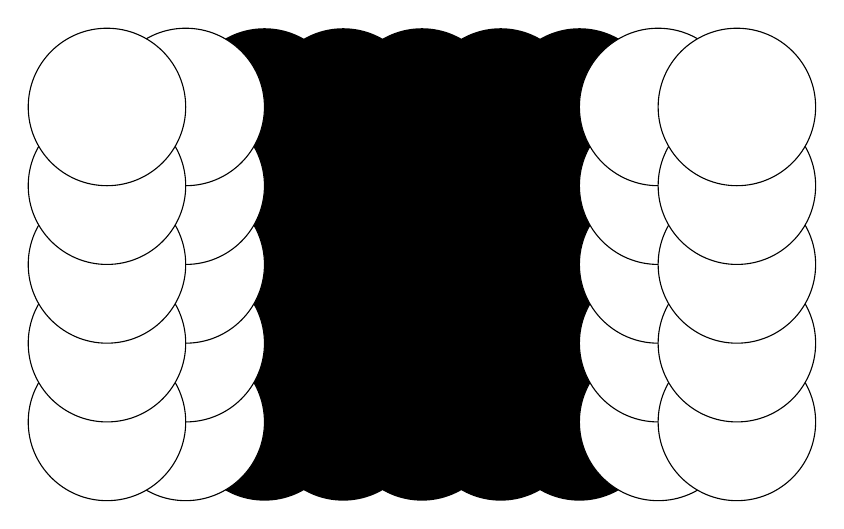
\begin{tikzpicture}
            \draw[very thin, step=1] (0,0) grid(4,4);
            \draw[very thin, dashed,step=1] (-1,0) grid(-2.5,4);
            \draw[very thin, dashed,step=1] (5,0) grid(6.5,4);
            \foreach \x in {0,...,4}{
                \foreach \y in {0,...,4}{
                    \fill (\x,\y) circle(\radius);
                }
            }
            \foreach \x in {-1,-2,5,6}{
                \foreach \y in {0,...,4}{
                    \filldraw[fill=white] (\x,\y) circle(\radius);
                }
            }

        \end{tikzpicture}
        \caption{Normally, one processor only has a local lattice and no data from the neighboring sub-lattices. An empty copy of the sub-lattice is made, to store the shifted lattice.}
    \end{subfigure}
    \begin{subfigure}{\textwidth}
        \centering
        \begin{tikzpicture}
            % Motion
            \draw[very thin, step=1] (0,0) grid(4,4);
            \draw[very thin, dashed,step=1] (-1,0) grid(-2.5,4);
            \draw[very thin, dashed,step=1] (5,0) grid(6.5,4);
            \foreach \x in {0,...,4}{
                \foreach \y in {0,...,4}{
                    \fill (\x,\y) circle(\radius);
                }
            }
            \foreach \x in {-1,-2,5,6}{
                \foreach \y in {0,...,4}{
                    \filldraw[fill=white] (\x,\y) circle(\radius);
                }
            }
            \foreach \x in {0,...,5}{
                \foreach \y in {0,...,4}{
                    \draw (\x,\y) ++(\outbend:\sepradius) coordinate(A);
                    \draw (\x-1,\y) ++(\inbend:\sepradius) coordinate (B);
                    \path[->] (A)  edge[bend right=\inbend] (B);
                }
            }
            \foreach \x in {0,4}{
                \draw (\x-\ovalspacing,-\radius) coordinate (A);
                \draw (A) ++(0,4+2*\radius) coordinate (B);
                \draw (\x+\ovalspacing,-\radius) coordinate (C);
                \draw (C) ++(0,4+2*\radius) coordinate (D);
                \draw[gray] (A) -- (B);
                \draw[gray] (C) -- (D);
                \draw[gray] (A) arc(180:360:\ovalspacing);
                \draw[gray] (D) arc(0:180:\ovalspacing);
            }
        \end{tikzpicture}
        \caption{The shifted lattice is filled with the neighboring links, some of which are received by the ``forward'' neighbor (so some are sent as well to the ``backward'' neighbor)}
        \label{subfig:shift}
    \end{subfigure}
    \begin{subfigure}{\textwidth}
        \centering
        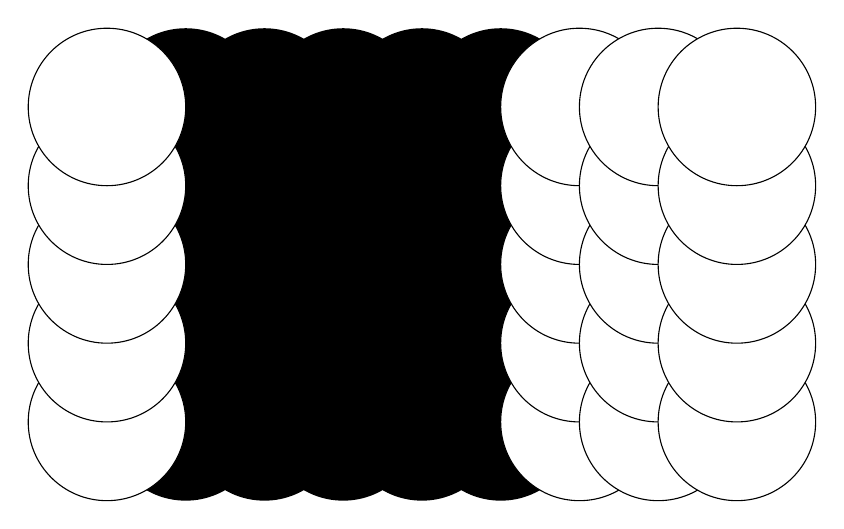
\begin{tikzpicture}
            \draw[very thin, step=1] (0,0) grid(4,4);
            \draw[very thin, dashed,step=1] (-1,0) grid(-2.5,4);
            \draw[very thin, dashed,step=1] (5,0) grid(6.5,4);
            \foreach \x in {-1,...,3}{
                \foreach \y in {0,...,4}{
                    \fill (\x,\y) circle(\radius);
                }
            }
            \foreach \x in {-2,4,5,6}{
                \foreach \y in {0,...,4}{
                    \filldraw[fill=white] (\x,\y) circle(\radius);
                }
            }
        \end{tikzpicture}
        \caption{The shifted lattice is now a local object mapped with the same indices as the original one. A site-by-site multiplication is now possible between the original and the shifted lattices.}
    \end{subfigure}
    \caption{Parallelization scheme based on lattice shifts. When, for example in the staples computation, a link needs to be multiplied by a neighboring one, a new lattice is created. It is filled with the shifted link, which is fetched either from the local sub-lattice if it is in the central region, or from the neighbors if it is on the edge. This schematic drawing shows how a shift along the ``right'' direction is performed. A new lattice containing the data of the target link is created by filling it with the target links. The circled regions in \cref{subfig:shift}, the edges, are shared using MPI by first creating a ``buffer'' of the shape of the edge (it is a cube in the real simulation) and it is sent in a single message to the neighbor which unpacks it in the right location. The new lattice is the multiplied with the original one on a site by site basis, which now is only a local operation.}
    \label{fig:shift}
\end{figure}

The data to be shifted is on the order of hundreds of kilobytes, which takes some time to be sent by MPI. An optimization that has been implemented is then to rewrite the algorithm in order to use non-blocking communications, first instantiating a send instruction non-blockingly, then shifting the inner points of the sub-lattice (which do not require links from the neighbors), waiting for the message from the neighbor to arrive, receiving the data from the neighbor and placing it in the buffer space.\\
This lattice shift operation has been implemented for the action derivative lattice and the gauge field itself. The massive reduction in communication overhead, compared to the single link exchange in \cref{sec:para_gen}, improved the scaling of the algorithm greatly, making this part of the problem much more efficient.

\subsection{Summary of the Parameters for the Gradient Flow}
As it has been done for the gauge field configuration generation algorithm, we report a summary of all free parameters of the program that performs the numerical integration of the gradient flow equation on the lattice configurations.

\begin{table}[!htb]
\begin{center}
\begin{tabular}{cl}
    Parameter & Description\\\hline
    $\beta$ & Coupling parameter of the Wilson Action, fixed by the input configuration\\
    $\epsilon$ & Runge-Kutta integration step\\
    $t_f^{MAX}$ & Maximum value of the flow time reached for every configuration. 
\end{tabular}
\label{FLOW:params}
\capt{Parameters for the numerical integration of the gradient flow equations on Yang-Mills gauge field configurations.}
\end{center}
\end{table}


\section{Structure and Tools}
The full code can be found on the web under the link \url{https://github.com/GioPede}, where both the code for the generation and the flow of gauge fields are hosted. The technical documentation is found at \url{https://giopede.github.io/LatticeYangMills/html/index.html} and \url{https://giopede.github.io/LatticeFlow/html/index.html}. As already mentioned the language of choice was \texttt{C++}, mainly because of the high-performance and abstraction level it  provides. An object-oriented structure has been used, as can be seen in 

\FIGURE{scheme class}. 

Notable tools that have been used that deserve a mention are \mpi, nlhoman/json \cite{_nlohmann/json} (used for easy input parameters handling via json files), CMake (for building the project) and Valgrind for function and memory profiling. 
